\documentclass[../main.tex]{subfiles}

\begin{document}
    \subsection{Predstavenie riešiteľského kolektívu}   
    Na riešení projektu sa podielali nasledovní študenti:

        Bc. Eva Štalmachová - študentka inžinierského študijného programu Robotika a Kybernetika na Ústave Robotiky a Kybernetiky FEI STU

        Bc. Marek Trebuľa - študent inžinierského študijného programu Robotika a Kybernetika na Ústave Robotiky a Kybernetiky FEI STU

        Bc. Ján Urdianyk - študent inžinierského študijného programu Robotika a Kybernetika na Ústave Robotiky a Kybernetiky FEI STU

        Bc. Denis Vasko - študent inžinierského študijného programu Robotika a Kybernetika na Ústave Robotiky a Kybernetiky FEI STU

    \subsection{Plán projektu}   
    Vytvorili sme rozpis úloh na jednotlivé týždne semestra:
    \begin{enumerate}
    	\item Voľba témy. Určenie spôsobu komunikácie, dohodnutie stretnutí. 
    	\item Voľba vedúceho tímu, analýza problému, dohoda o obsahu riešenia. Zaučenie členov pre prácu s programom git. 
    	\item Štúdium literatúry zaoberajúcou sa danou problematikou.
    	\item Určenie prvotných úloh jednotlivých členov tímu.
    	\item Kontrola splnenia pridelených úloh, odvodenie ďalších úloh.
    	\item Dokumentácia vyriešených častí úlohy. A príprava prezentácie čiastočného riešenia.
    	\item Prezentácia čiastočného riešenia vedúcemu projektu, analýza kritiky vedúceho a syntéza nových úloh. 
    	\item Riešenie a dokumentácia nových úloh, konzultácia s vedúcim projektu.
    	\item Pokračovanie v riešení úloh z predchádzajúceho týždna.
    	\item Destilácia obsahu riešenia do formy prezentácie.
    	\item Vypracovanie posudku na konkurenčný projekt.
    	\item Prezentácia.
    \end{enumerate}

    \subsection{Dohodnuté metódy práce}   
    	\begin{itemize}
    		\item Pre projekt bude vytvorený repozitár na stránkach github.com, do ktorého bude každý z členov prispievať svoju časť riešenia.
    		\item Forma riešenia bude predpísaná šablónou, ktorou sa členovia budú riadiť pri štrukturovaní práce a dokumentácie.
            \item Dokumentácia bude vytvorená v dokumentačnom systéme LaTeX.
            \item Simulácie budú vytvorené v simulačnom prostredí Matlab/Simulink.
            \item Verzie riešenia budú spravované využitím programu git a jednotlivé verzie budú hostované na stránkach github.com ako súkromný repozitár.
            \item Pre zabezpečenie dodržania termínov sme zaviedli aj časové obmedzenia doby riešnia jednotlivých úloh pridelených členom skupiny.
    	\end{itemize}

    \subsection{Komunikácia a koordinácia projektu}
    	\begin{itemize}
    		\item Komunikácia s pánom prof. Murgašom prebieha počas naplánovaných stretnutí, alebo mailom.
    		\item Medzi členmi tímu prostredníctvom facebookovej skupiny, alebo osobne. 
            \item Neskôr väčšina komunikácie medzi členmi tímu prebiehala prostredníctvom programu MS teams, využitím textových správ ale aj videohovorov.
    	\end{itemize}

    \subsection{Kontrola rozhodnutí tímu}
    
    \subsection{Podrobné záznamy o stretnutí}
    Uvádzame vyhotovené zápisnice stretnutí, zápisnice vypracoval Bc. Marek Trebuľa.

    % 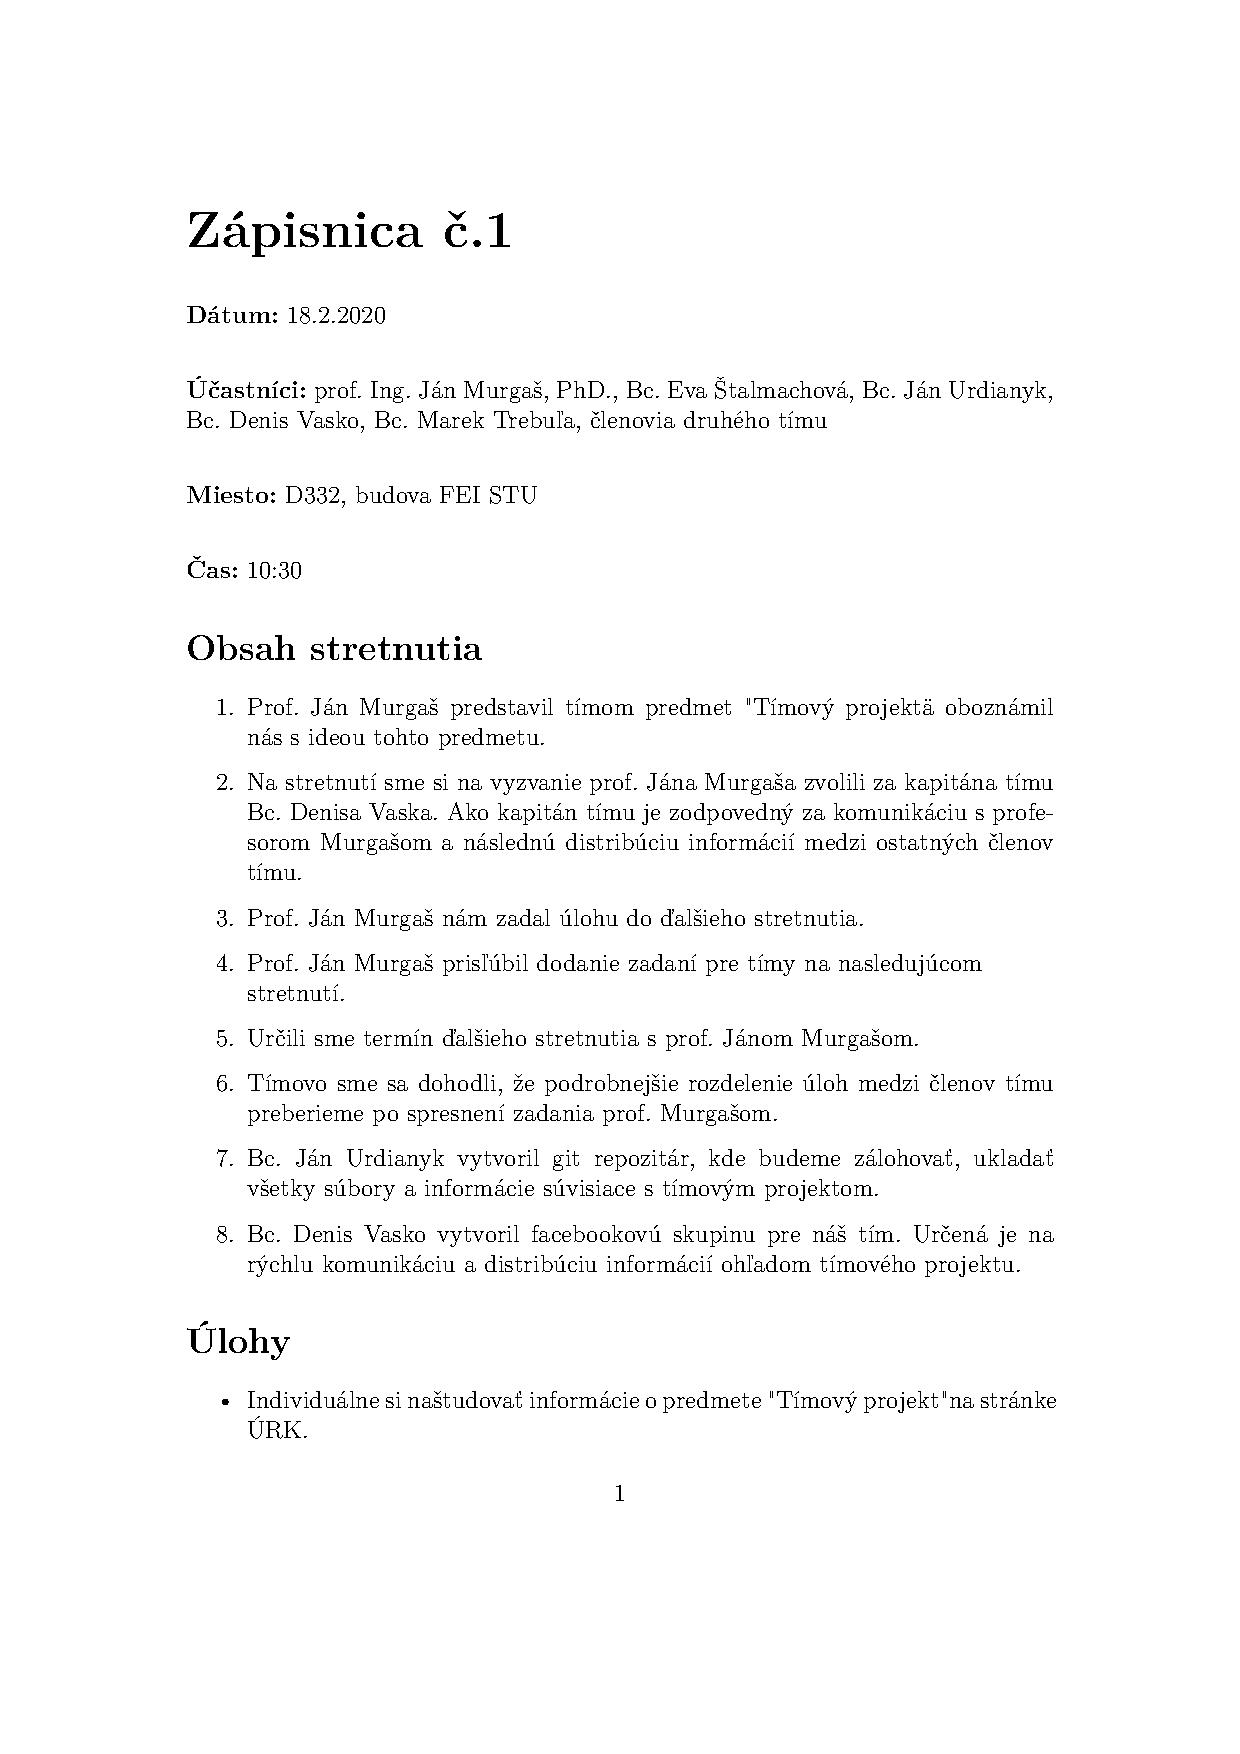
\includepdf{../../Zapisnice/Zapisnica1_18022020.pdf}
    % 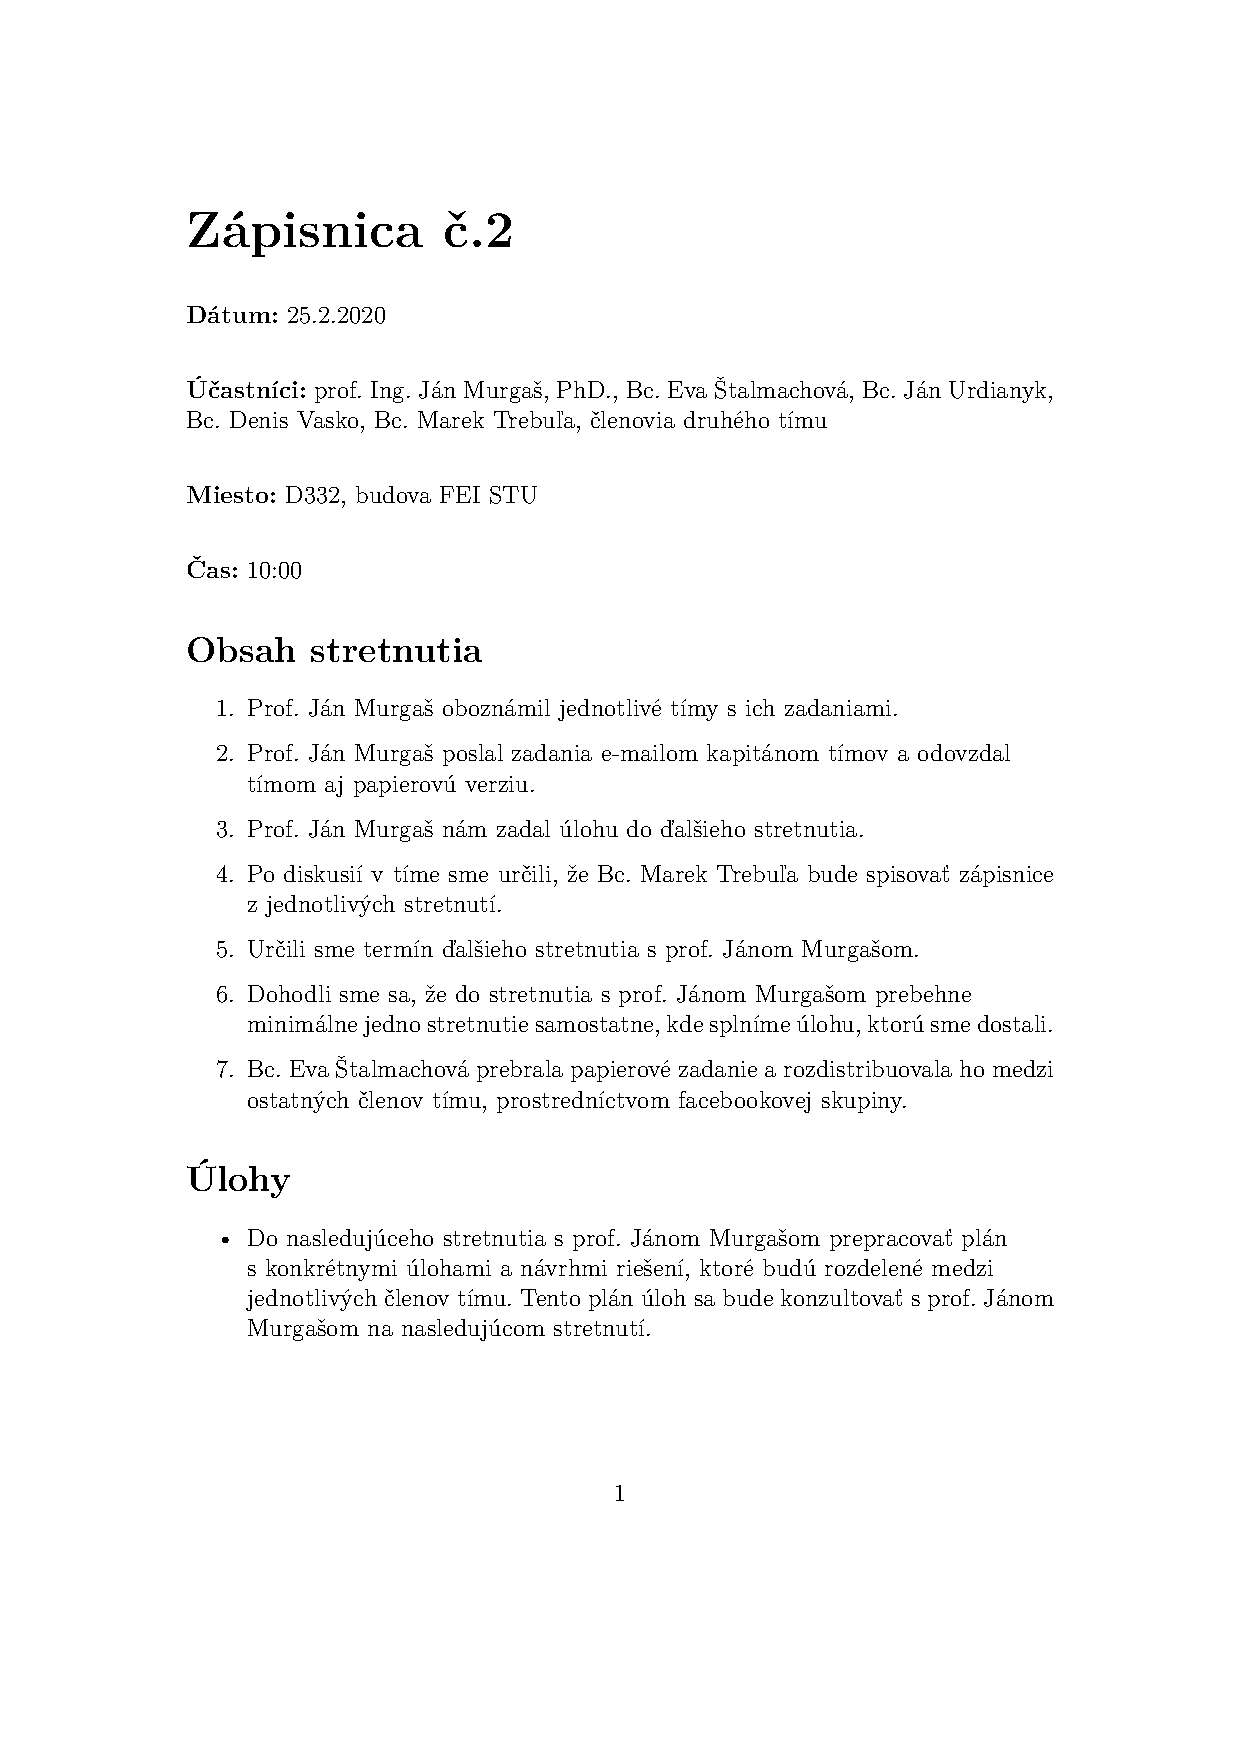
\includepdf{../../Zapisnice/Zapisnica2_25022020.pdf}
    % 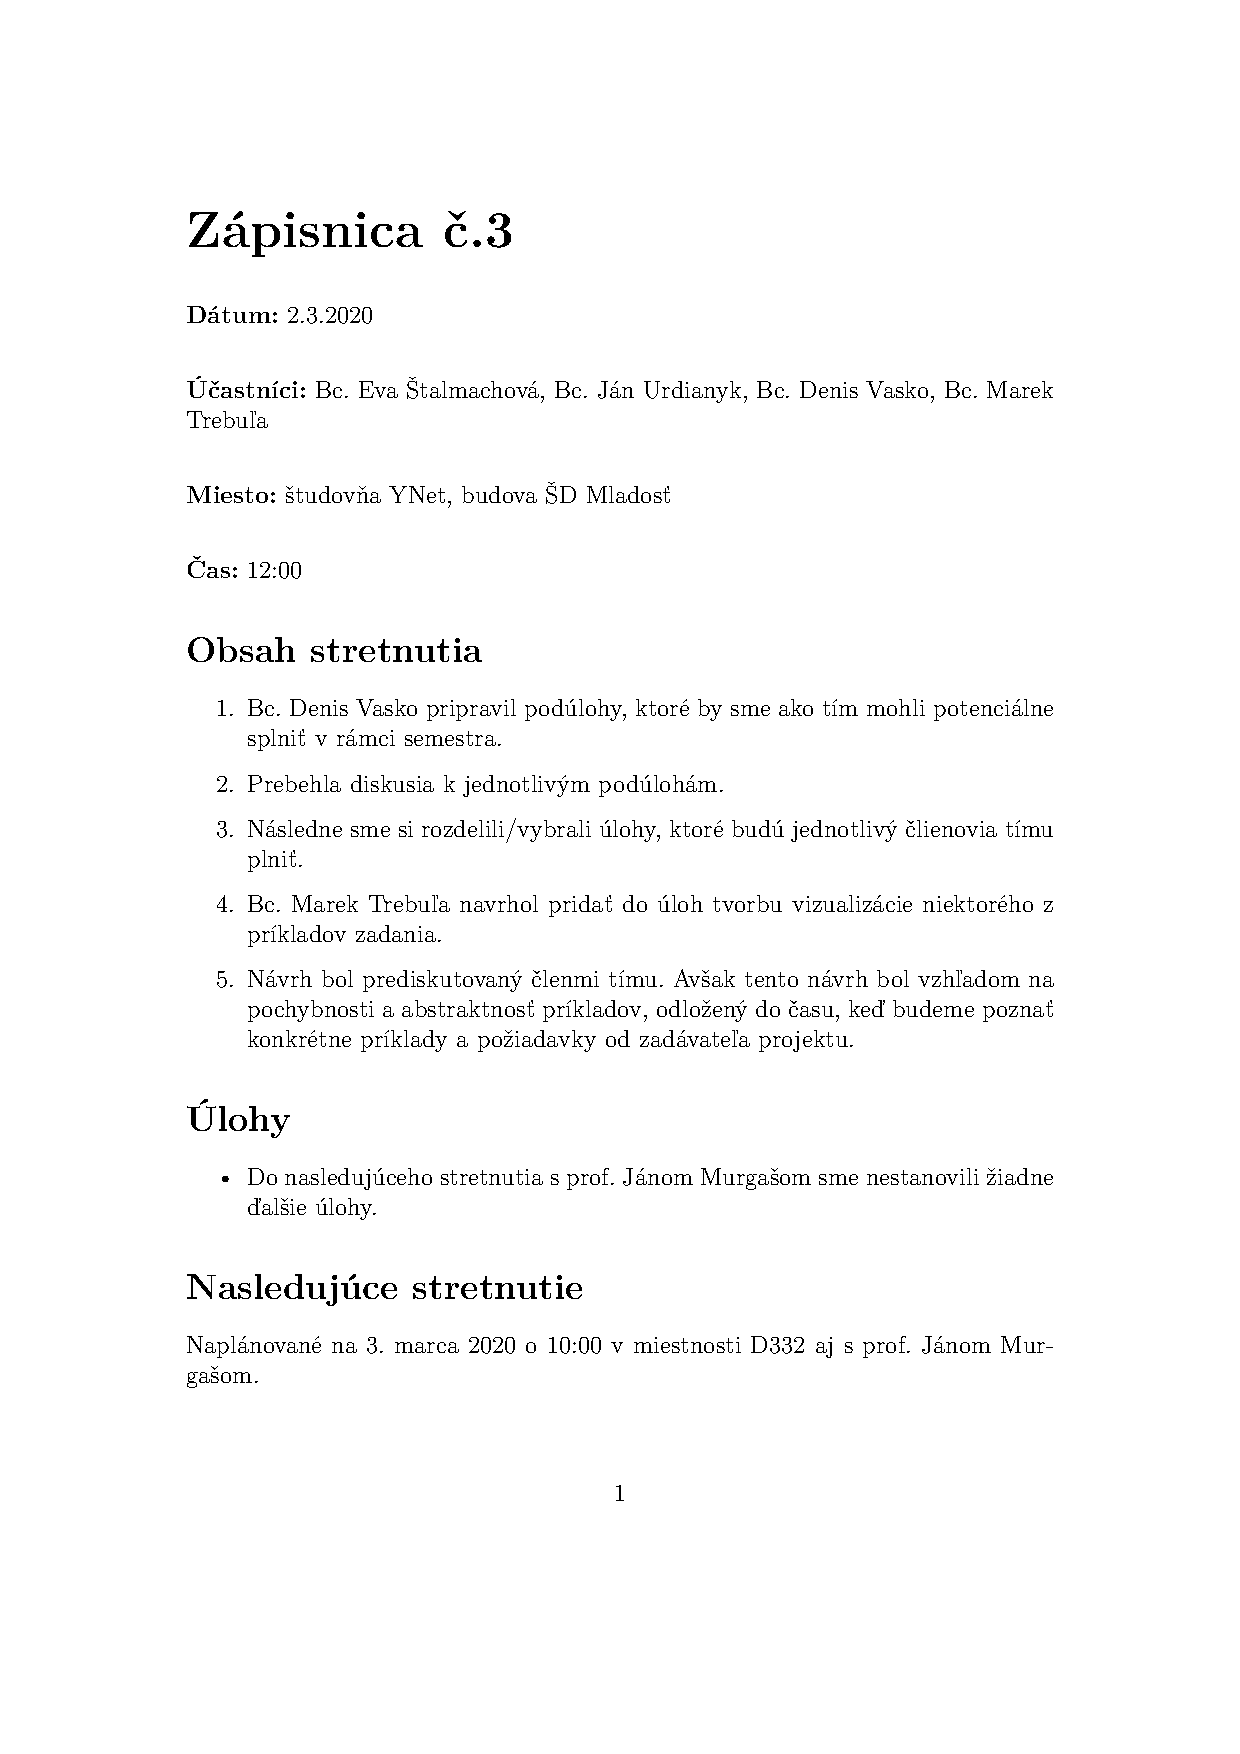
\includepdf{../../Zapisnice/Zapisnica3_02032020.pdf}
    % 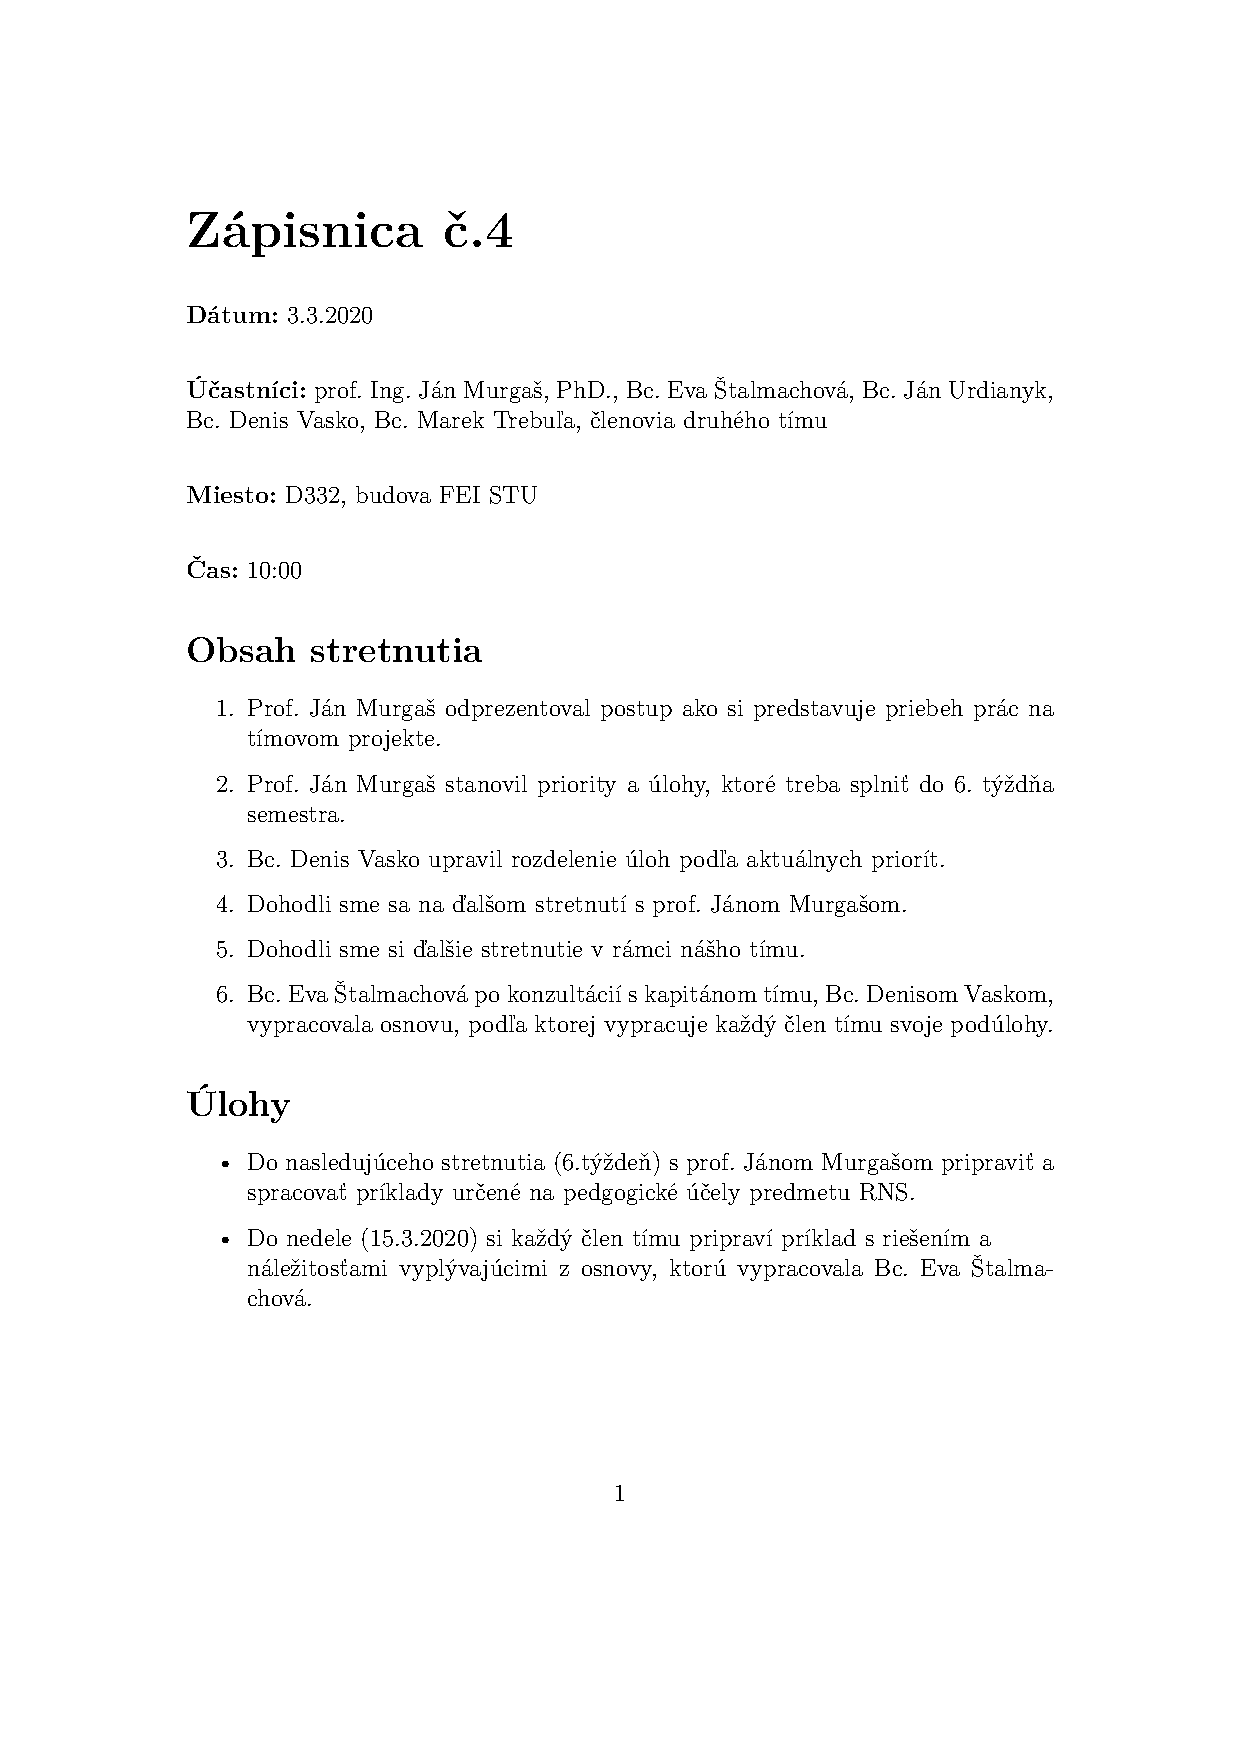
\includepdf{../../Zapisnice/Zapisnica4_03032020.pdf}
    % 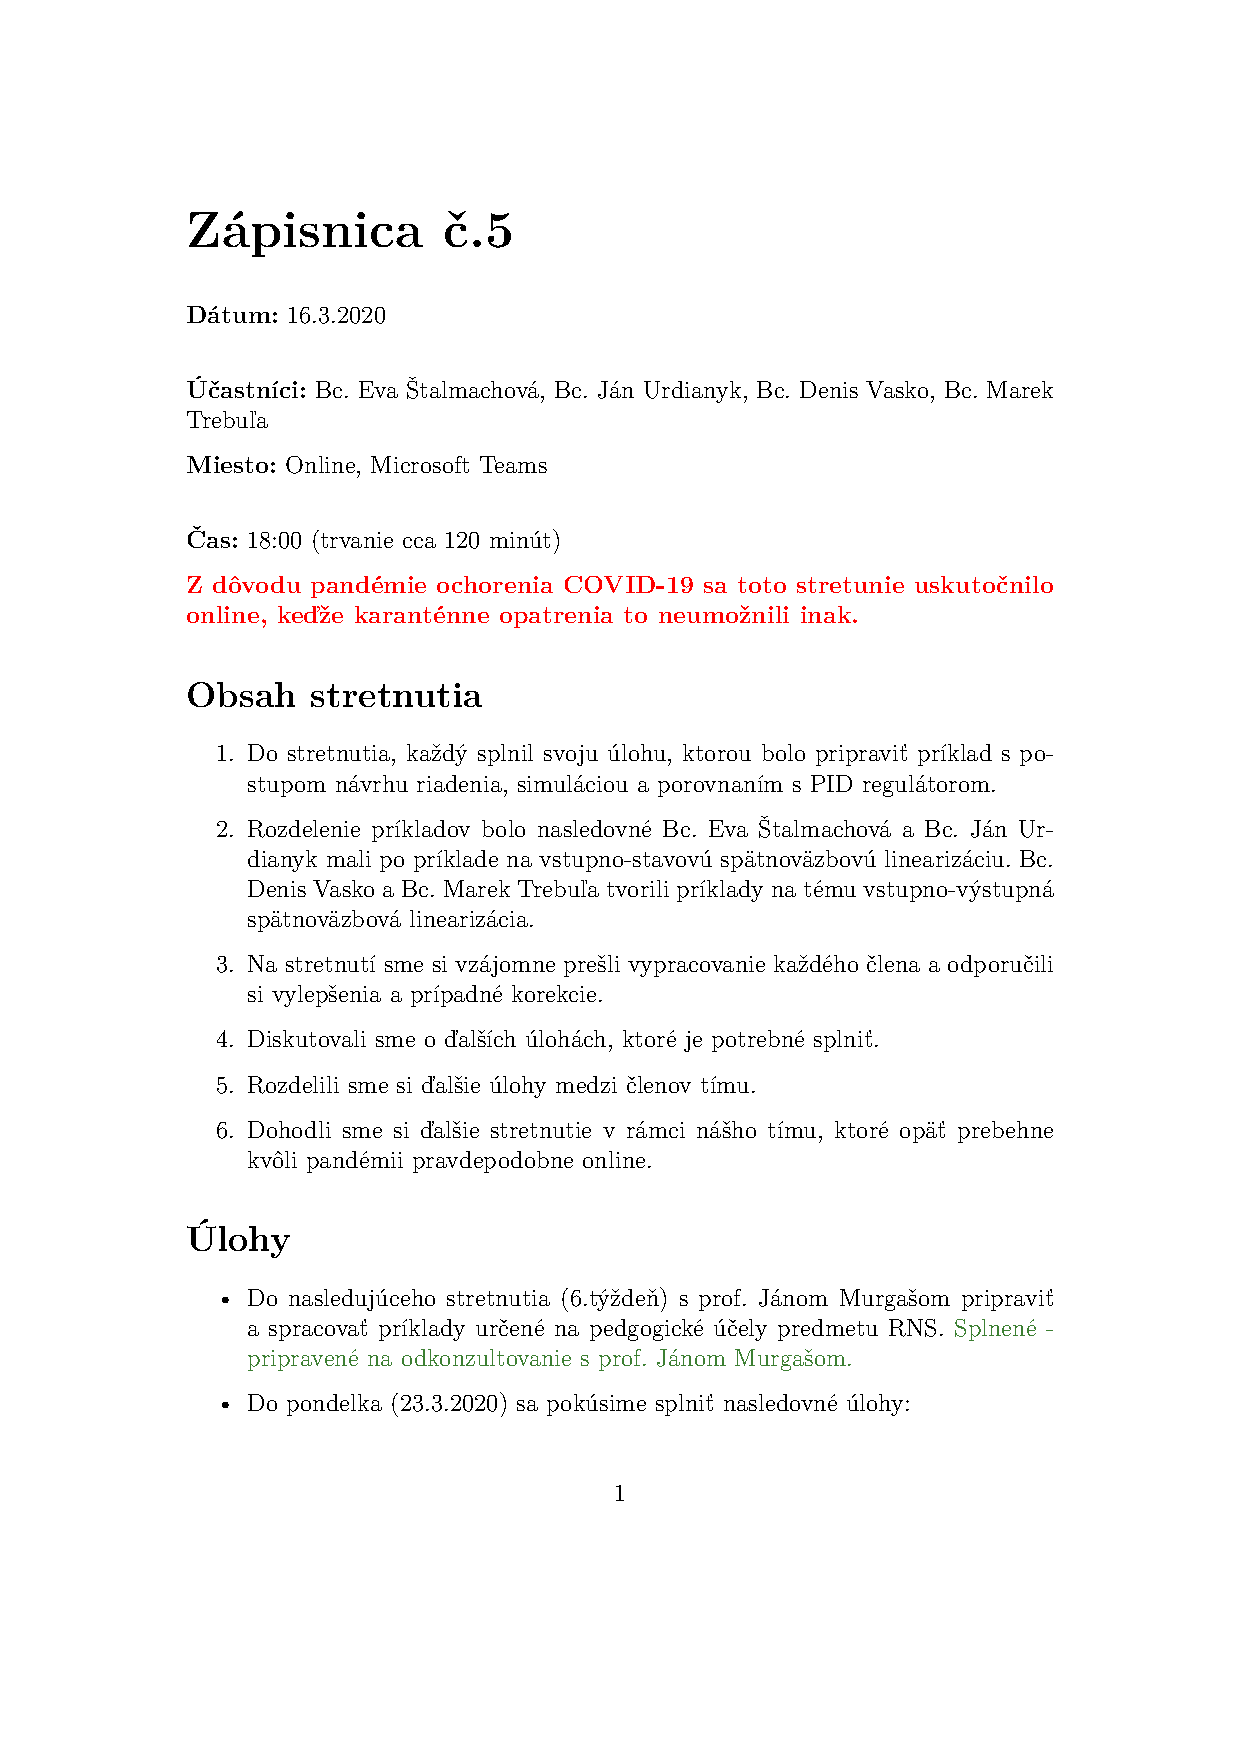
\includepdf{../../Zapisnice/Zapisnica5_16032020.pdf}
    % 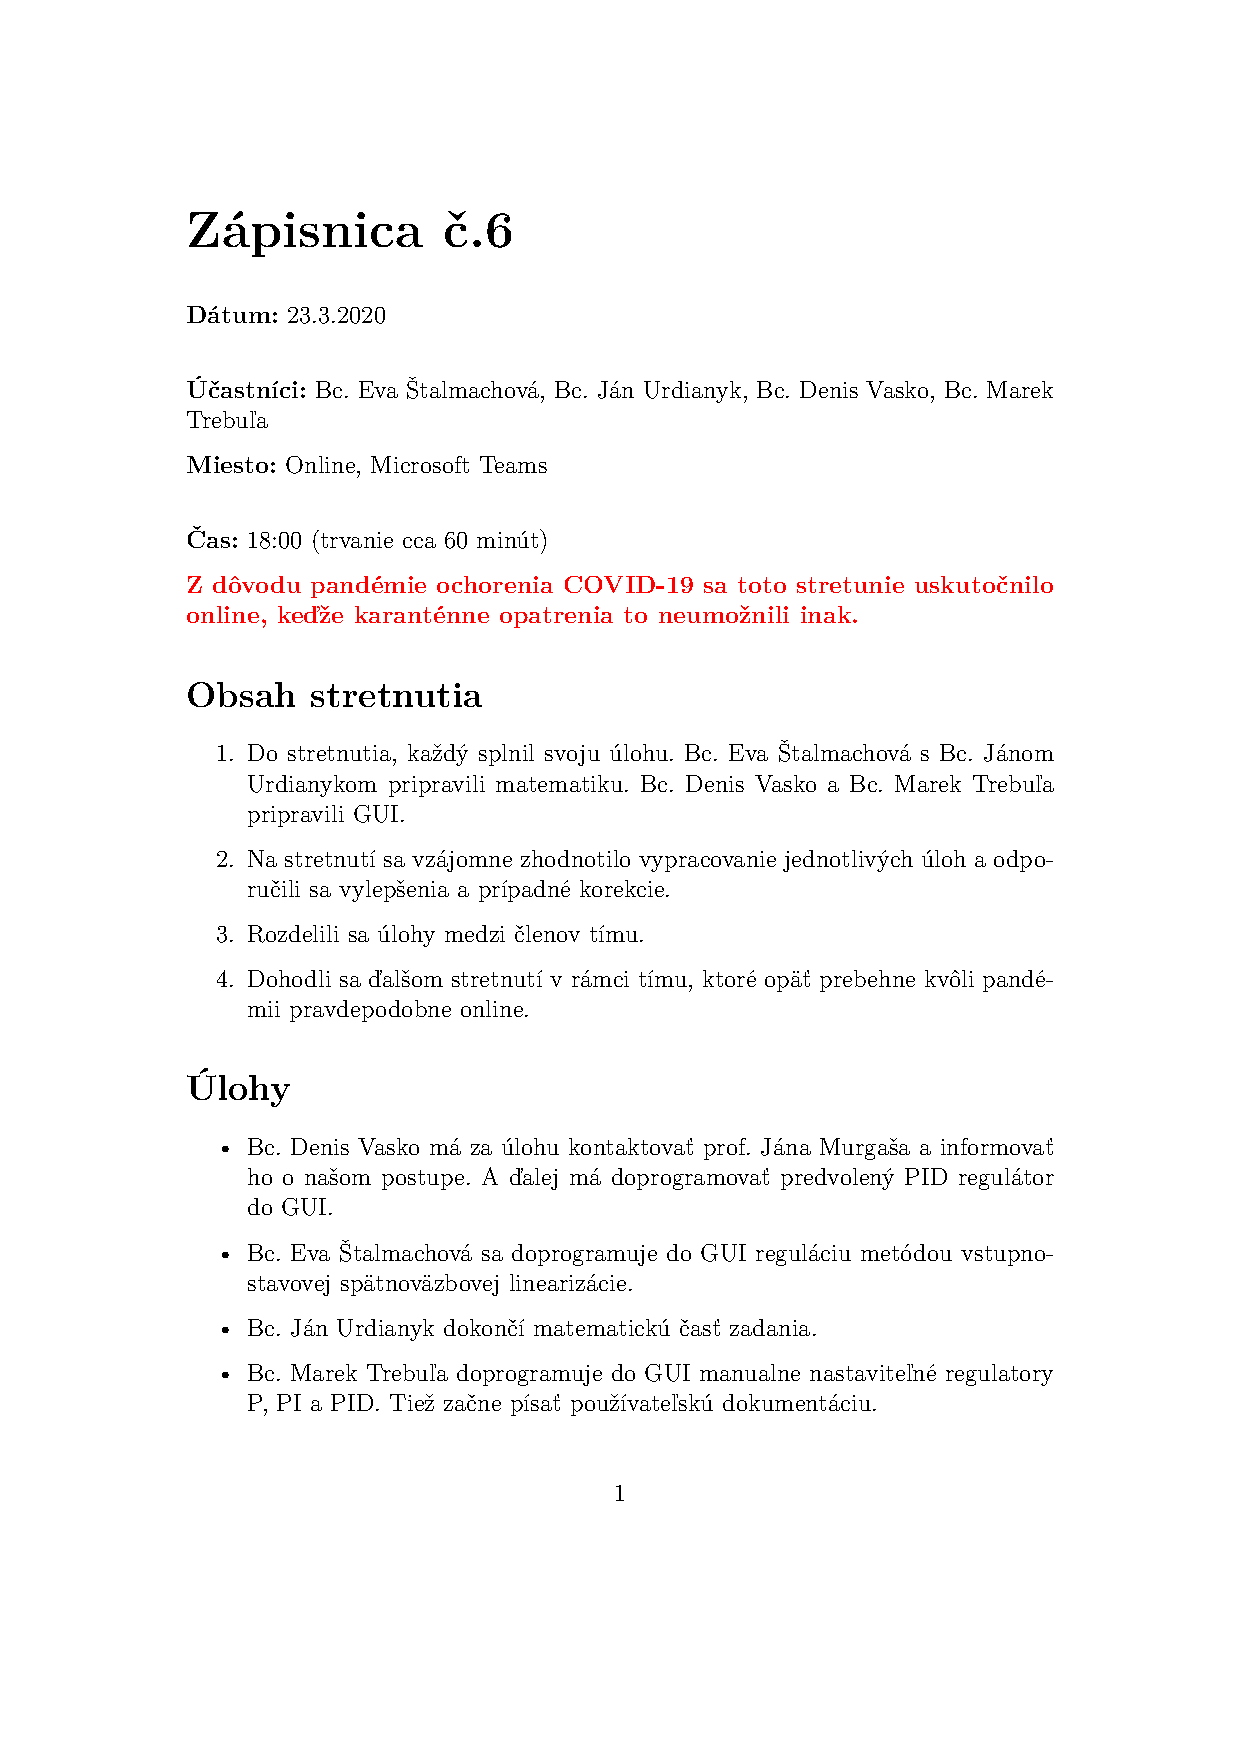
\includepdf{../../Zapisnice/Zapisnica6_23032020.pdf}
    % 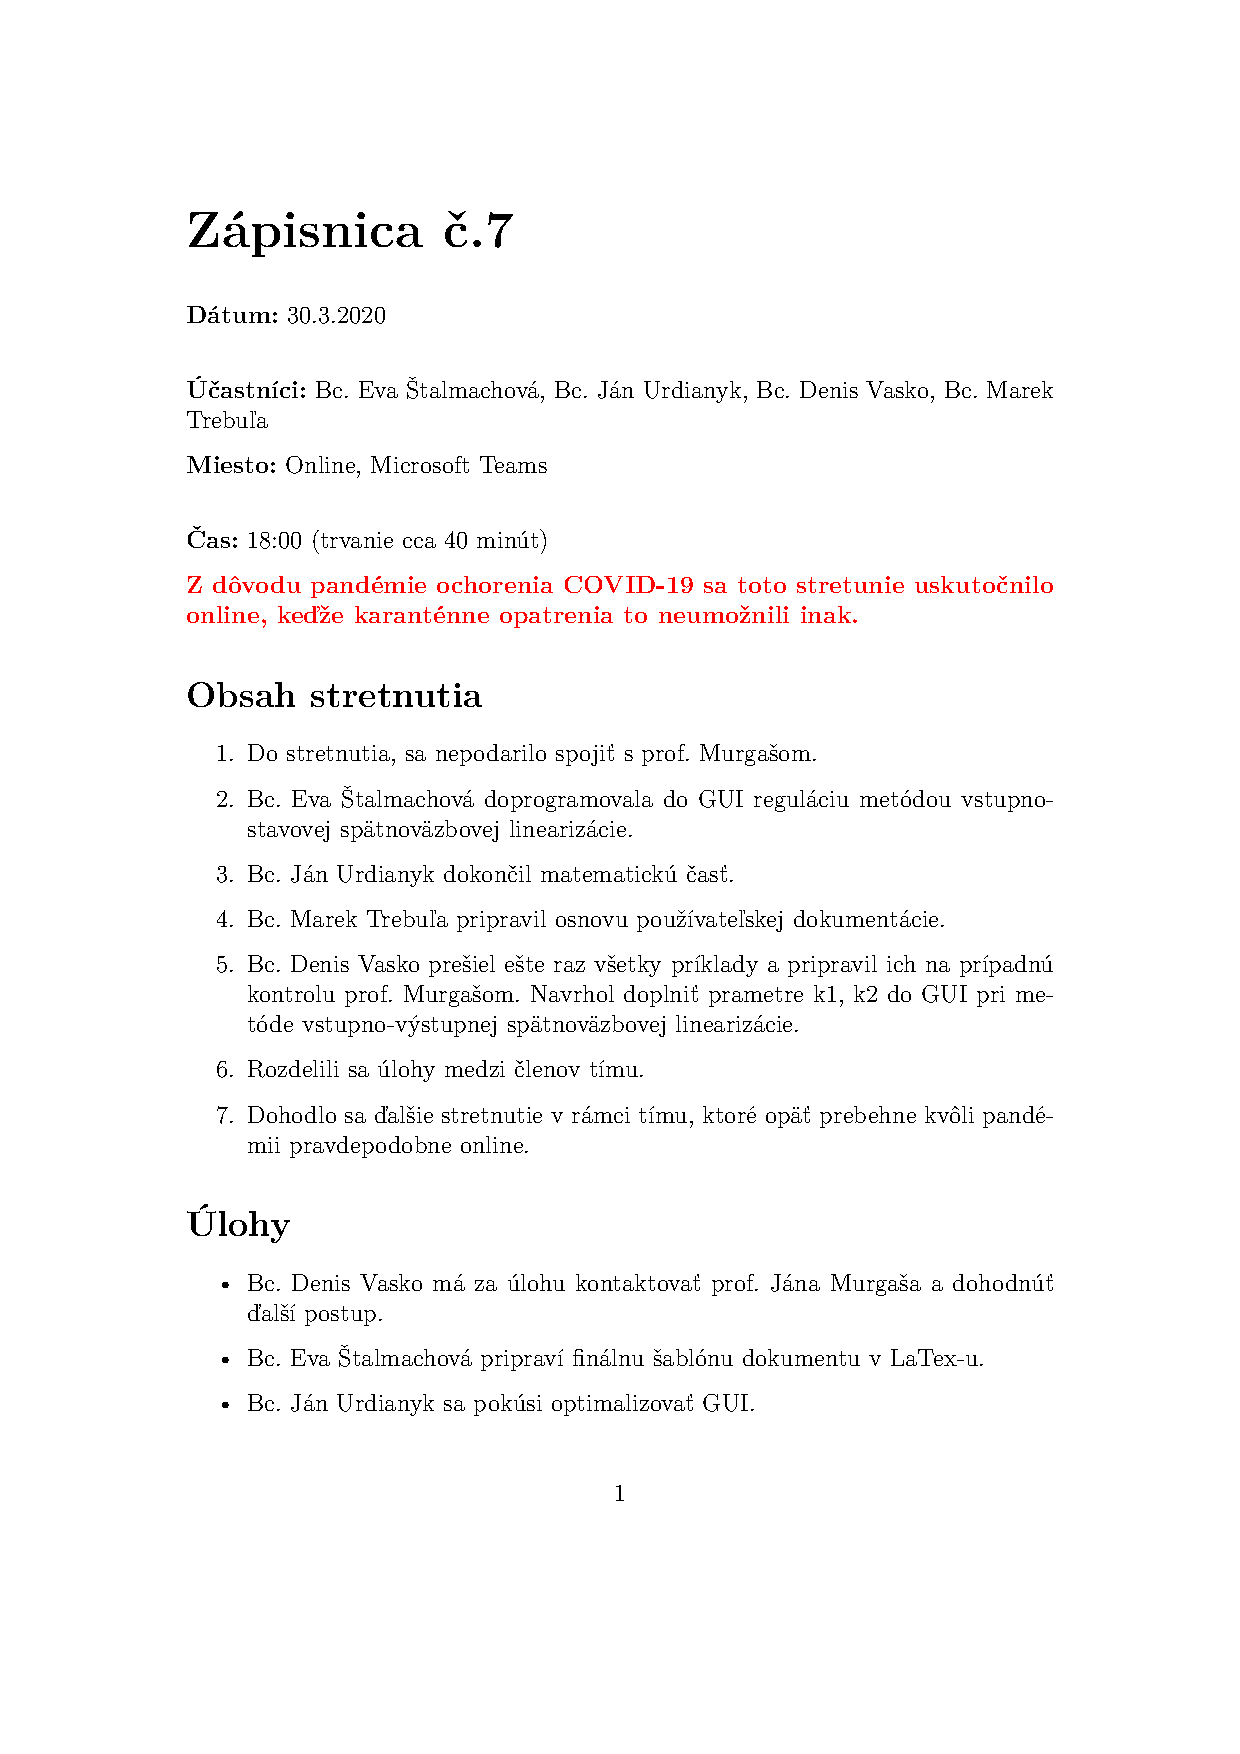
\includepdf{../../Zapisnice/Zapisnica7_30032020.pdf}
    % 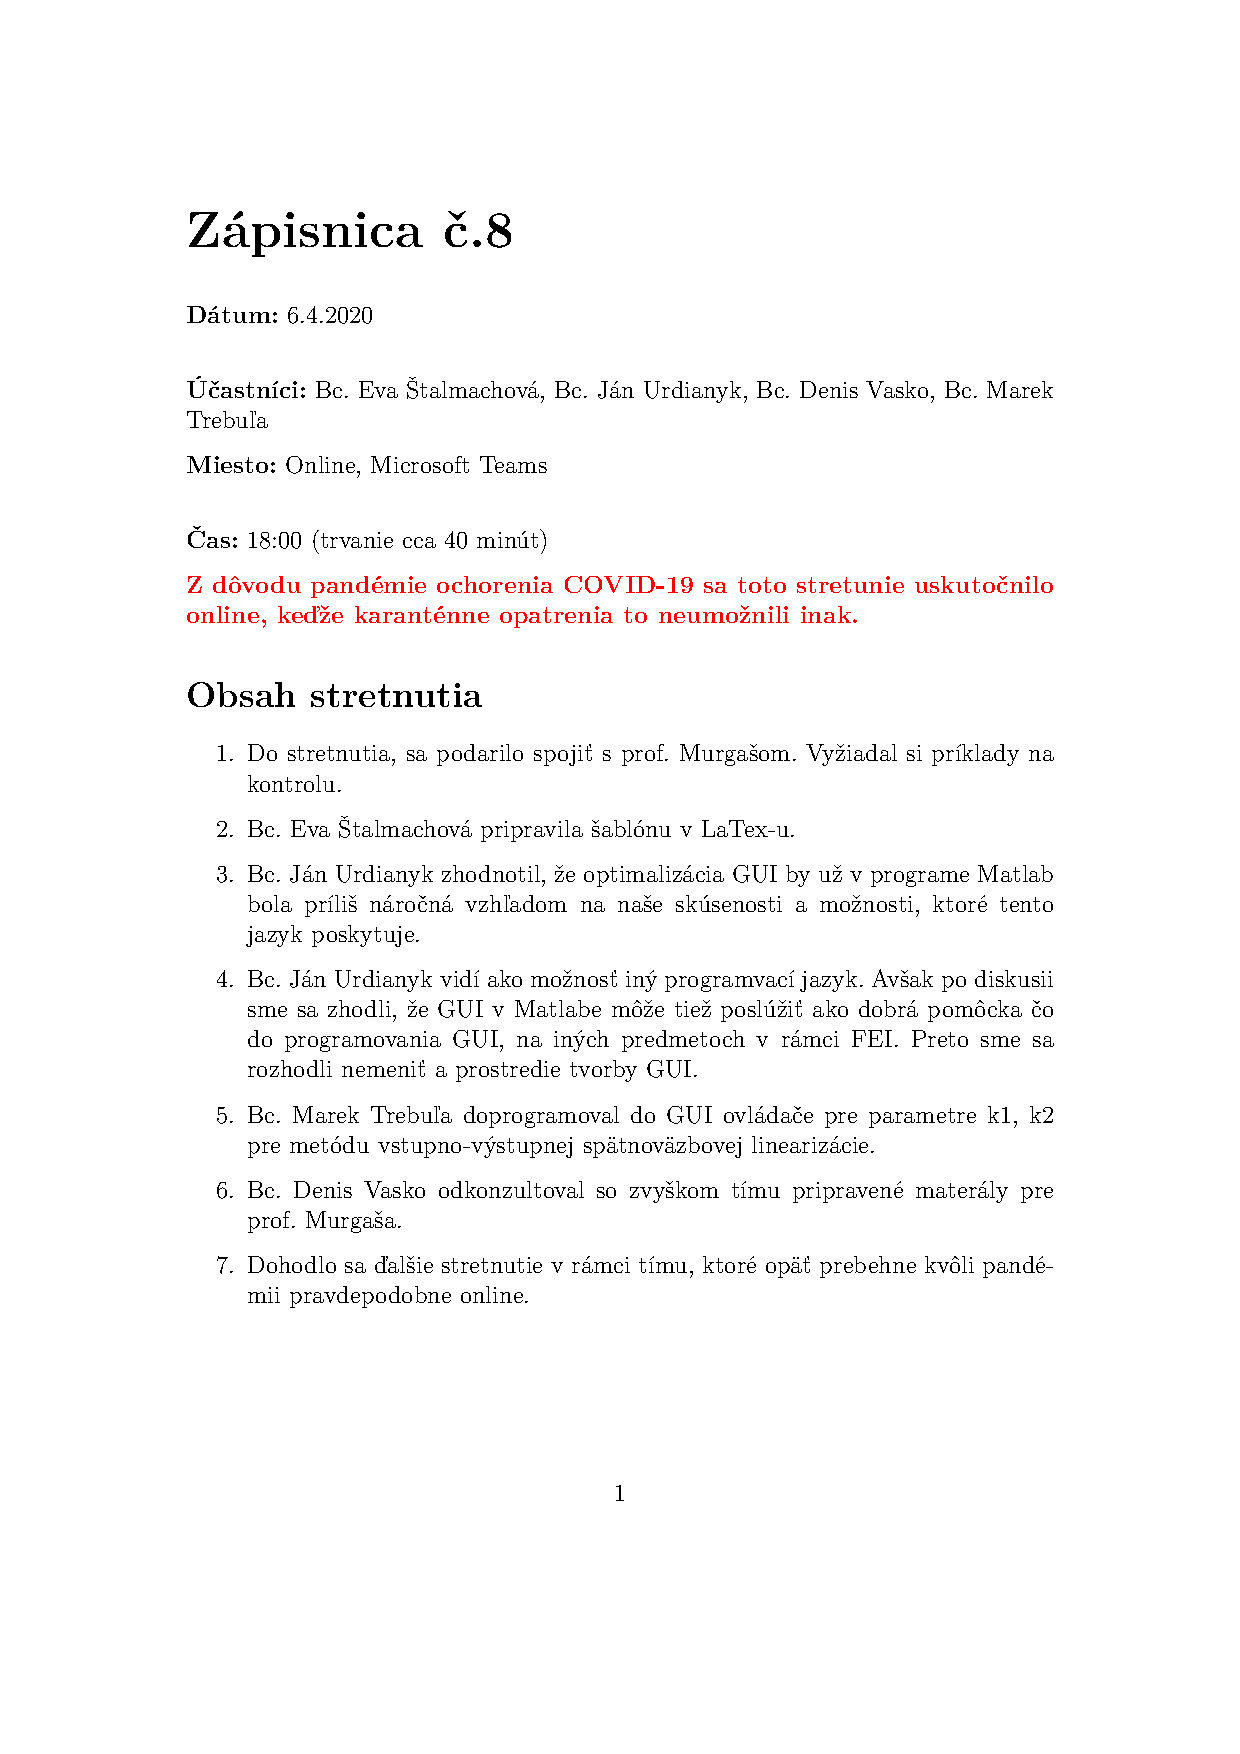
\includepdf{../../Zapisnice/Zapisnica8_06042020.pdf}
    % 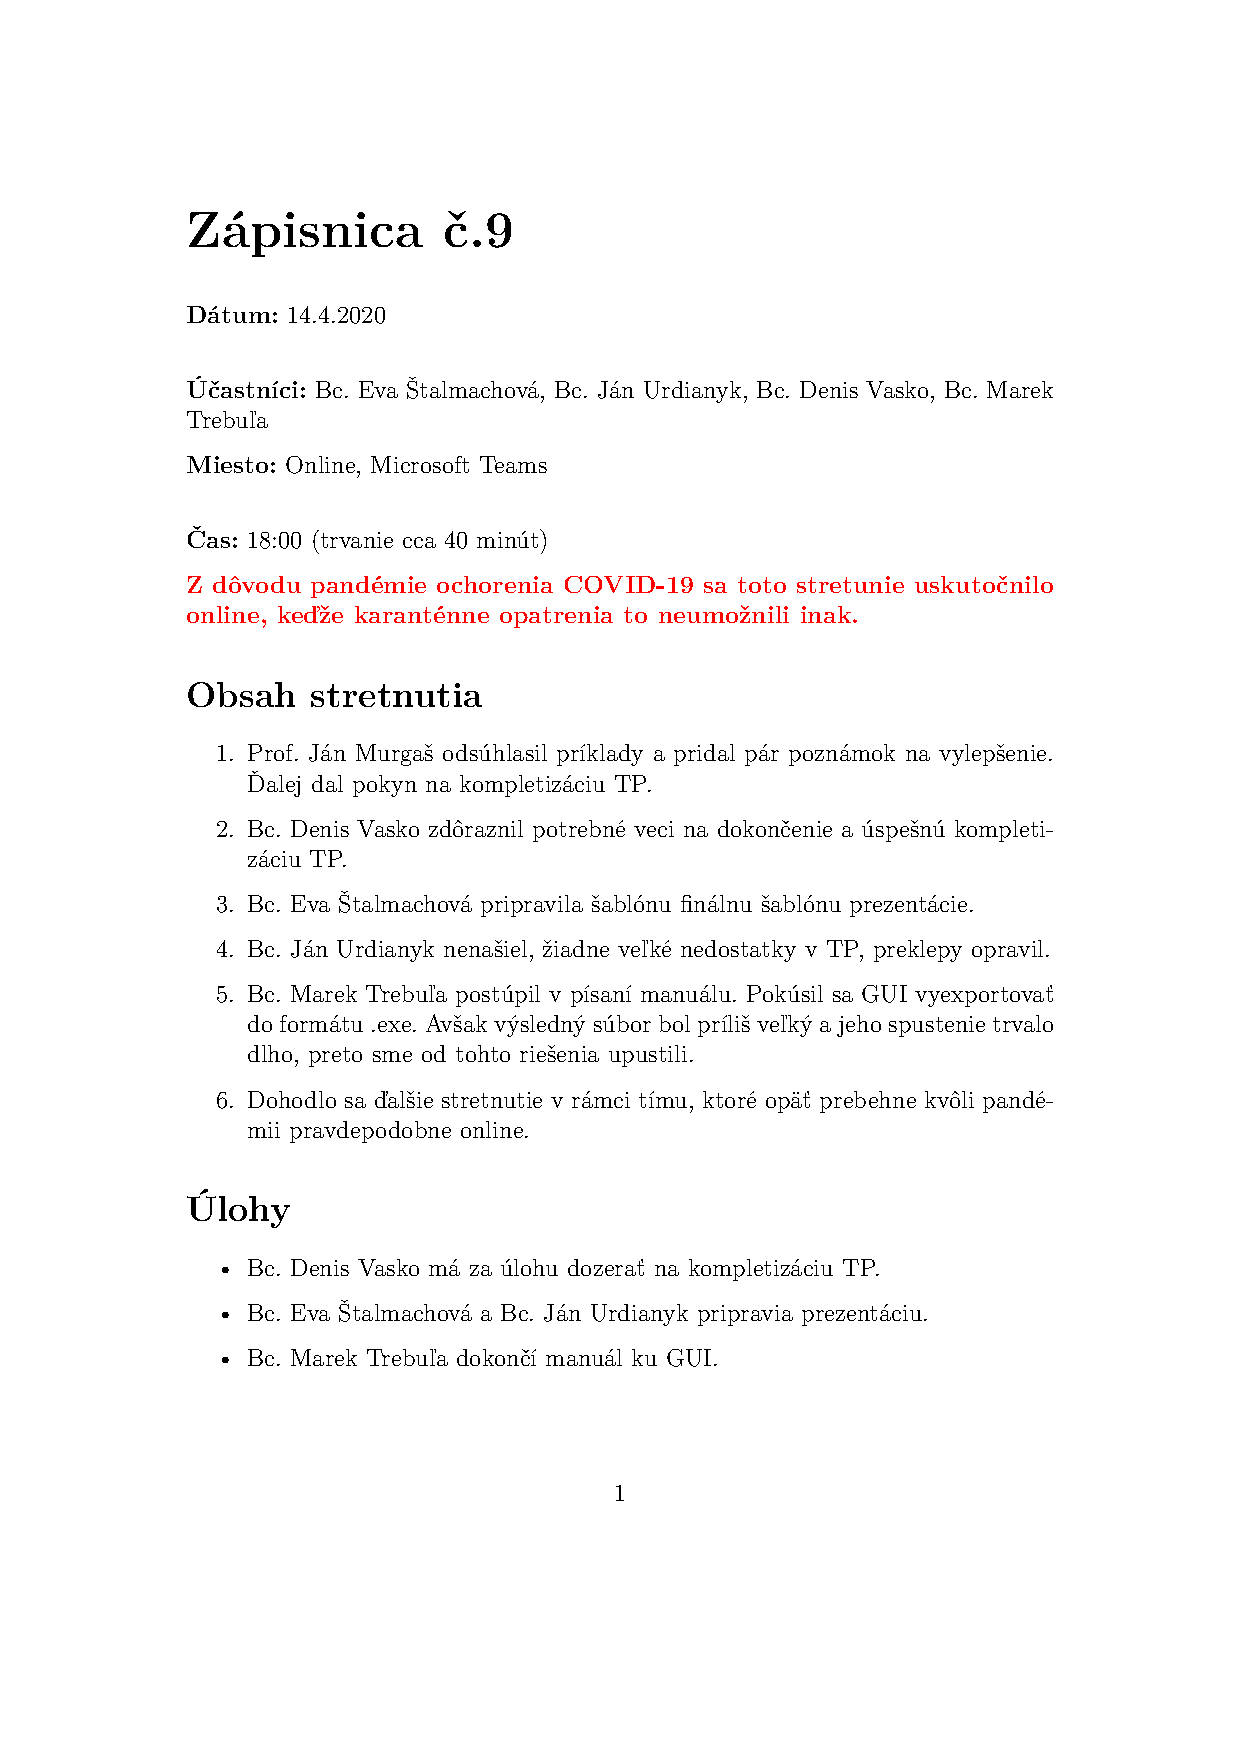
\includepdf{../../Zapisnice/Zapisnica9_14042020.pdf}

\end{document}
